%%% Template originaly created by Karol Kozioł (mail@karol-koziol.net) and modified for ShareLaTeX use

\documentclass[a4paper,11pt]{article}

\usepackage[T1]{fontenc}
\usepackage[utf8]{inputenc}
\usepackage{graphicx}
\usepackage{xcolor}
\usepackage[]{authblk}
\usepackage{subcaption}

\renewcommand\familydefault{\sfdefault}
\usepackage{tgheros}
\usepackage[defaultmono]{droidmono}

\usepackage{amsmath,amssymb,amsthm,textcomp}
\usepackage{enumerate}
\usepackage{multicol}
\usepackage{tikz}

\usepackage{geometry}
%\geometry{total={210mm,297mm},
%left=25mm,right=25mm,%
%bindingoffset=0mm, top=20mm,bottom=20mm}


\linespread{1.2}

\newcommand{\linia}{\rule{\linewidth}{0.5pt}}

% custom theorems if needed
\newtheoremstyle{mytheor}
    {1ex}{1ex}{\normalfont}{0pt}{\scshape}{.}{1ex}
    {{\thmname{#1 }}{\thmnumber{#2}}{\thmnote{ (#3)}}}

%\theoremstyle{mytheor}
%\newtheorem{defi}{Definition}

% my own titles
\makeatletter
\renewcommand{\maketitle}{
\begin{center}
\vspace{1ex}
{\LARGE \textsc{\@title}}
\vspace{0.5ex}
\linia\\
\@author \hfill \@date
%\@personNumber \hfill \@email
\vspace{3ex}
\end{center}
}
\makeatother
%%%

% custom footers and headers
\usepackage{fancyhdr}
\pagestyle{fancy}
\lhead{}
\chead{}
\rhead{}
\lfoot{HW 1}
\cfoot{}
\rfoot{Page \thepage}
\renewcommand{\headrulewidth}{0pt}
\renewcommand{\footrulewidth}{0pt}
%

% code listing settings
\usepackage{listings}
\lstset{
    language=Python,
    basicstyle=\ttfamily\small,
    aboveskip={1.0\baselineskip},
    belowskip={1.0\baselineskip},
    columns=fixed,
    extendedchars=true,
    breaklines=true,
    tabsize=4,
    prebreak=\raisebox{0ex}[0ex][0ex]{\ensuremath{\hookleftarrow}},
    frame=lines,
    showtabs=false,
    showspaces=false,
    showstringspaces=false,
    keywordstyle=\color[rgb]{0.627,0.126,0.941},
    commentstyle=\color[rgb]{0.133,0.545,0.133},
    stringstyle=\color[rgb]{01,0,0},
    numbers=left,
    numberstyle=\small,
    stepnumber=1,
    numbersep=10pt,
    captionpos=t,
    escapeinside={\%*}{*)}
}

%%%----------%%%----------%%%----------%%%----------%%%

\begin{document}

\title{Hw 1: Spatial Pyramid Matching for Scene Classification}

\author{Avinash Kommineni, 50248877} 
%\personNumber{50248877}
%\email{akommineni@buffalo.edu}
%\personNumber {50248877}
%\email{akommineni@buffalo.edu}
\date{\today}

\maketitle

\section*{Problem 1.0}

Each of the above 20 images are filters in their respective colours with increase in size. So the first row searches for reddish yellow patches surrounded by blue with decreasing granularity. The same with 2nd row. The $3^{rd}$ and $4^{th}$ rows serves the purpose of edge detection. Since there has been an increase in the size of the filters from left to right, the resultant image (filtered  image) looks more smooth/ blurred out than the one to it's left. \\
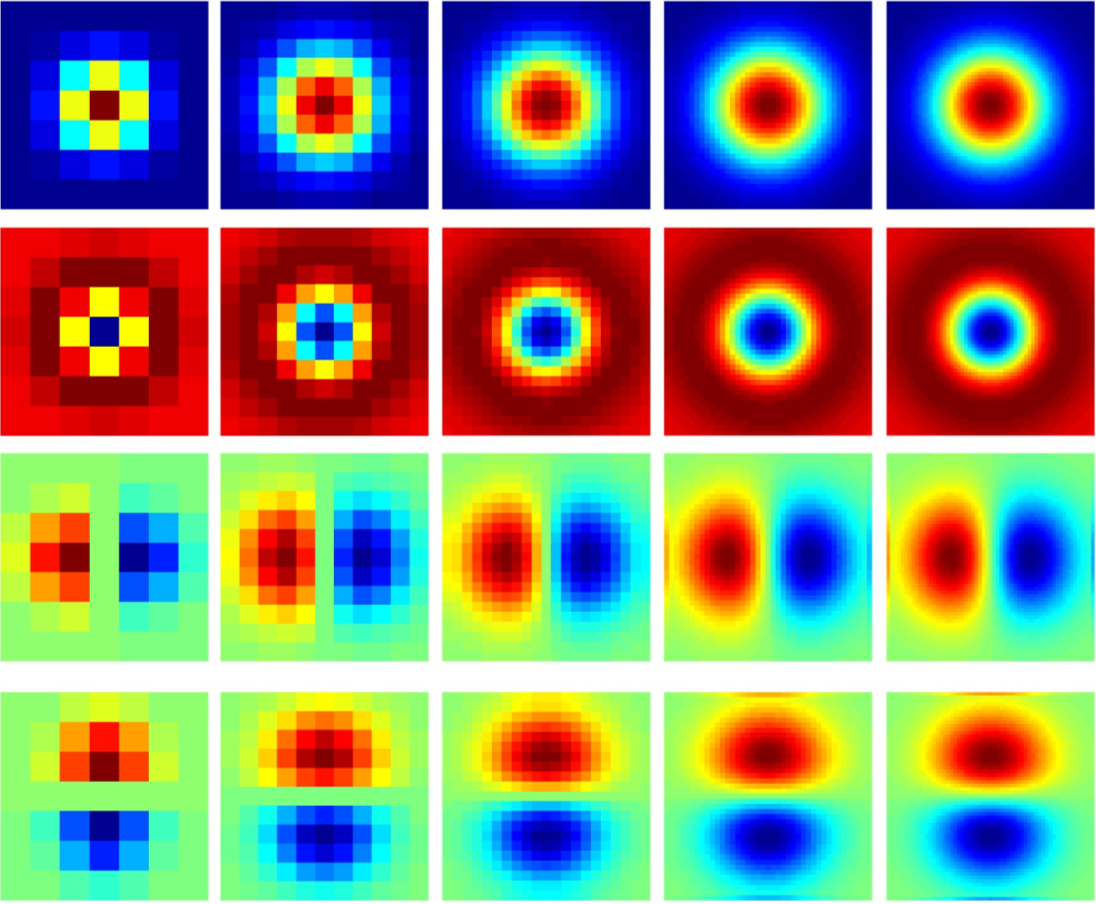
\includegraphics[width=\textwidth]{filters}\\
This is evident from the below image.\\
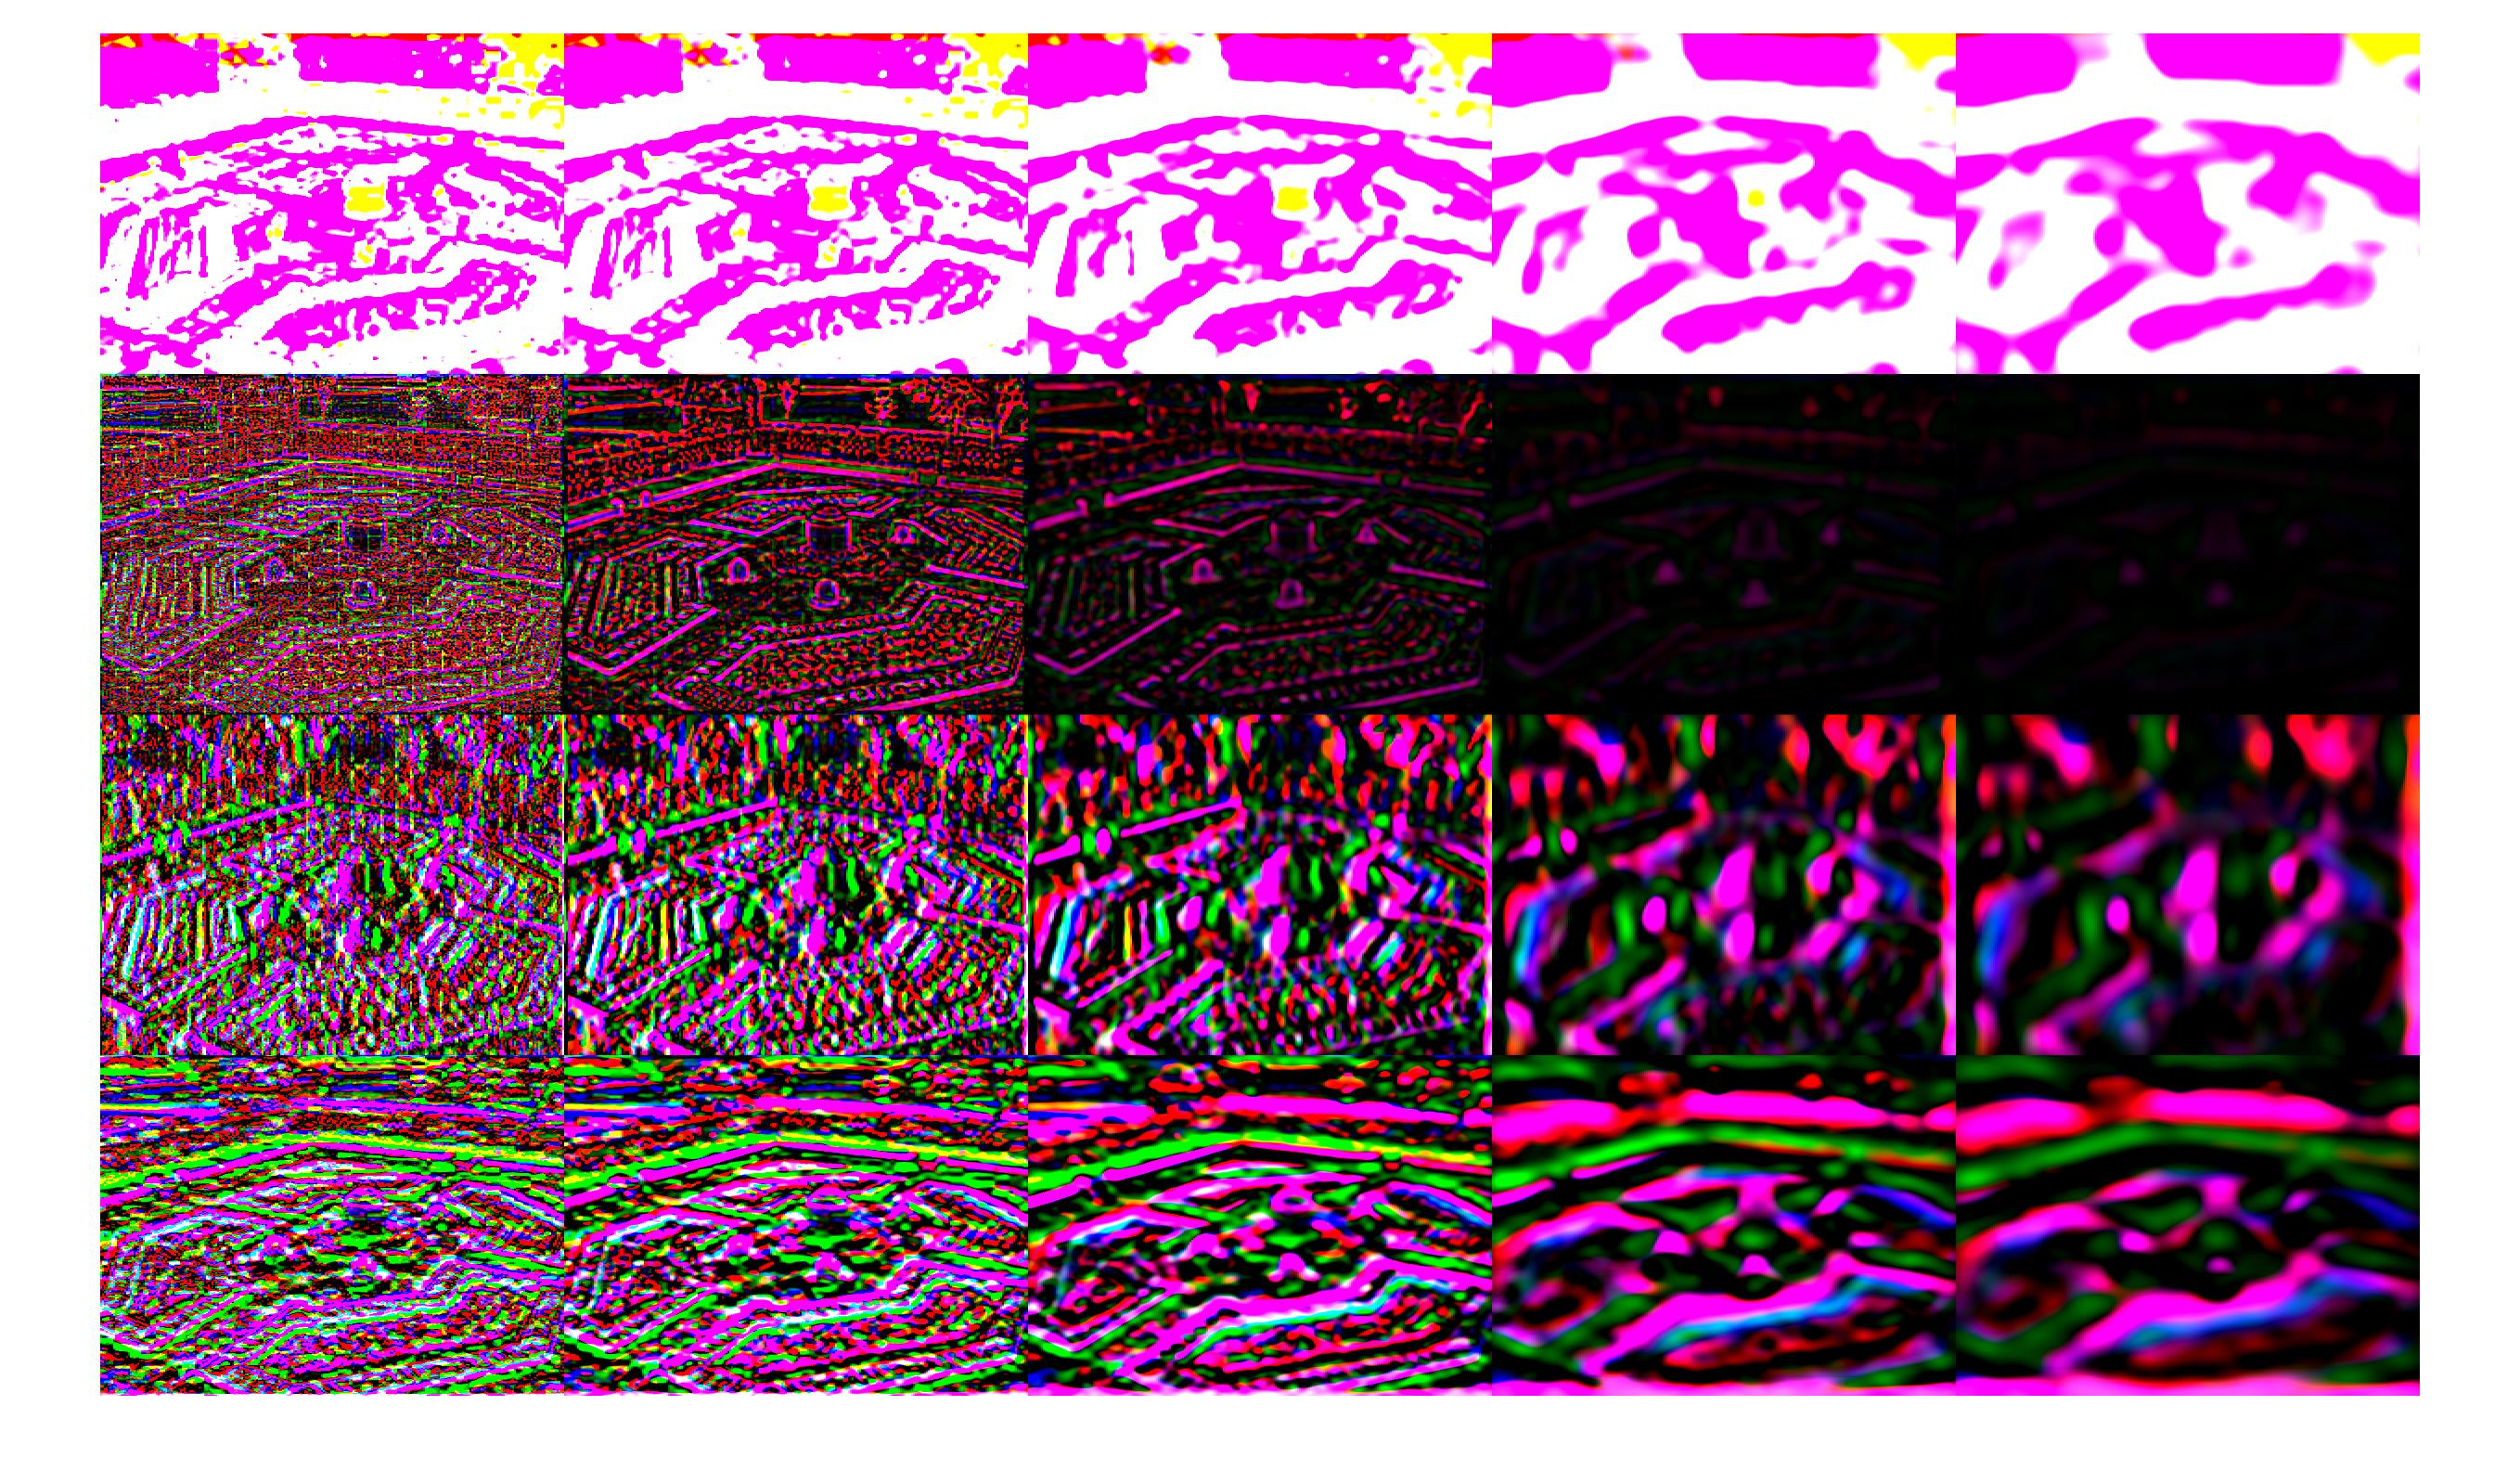
\includegraphics[width=\textwidth]{Montage1}
The  $3^{rd}$ and $4^{th}$ rows are acting as vertical and horizontal edge detectors respectively and the $1^{st}$ and $2^{nd}$ as  more of blob detectors.\\
\vfill
\section*{Problem 1.1}
Below dsiplayed are the actual images followed by their respective filter responses.
\begin{center}
\includegraphics[width=11cm]{release/matlab/fig4}
\end{center}
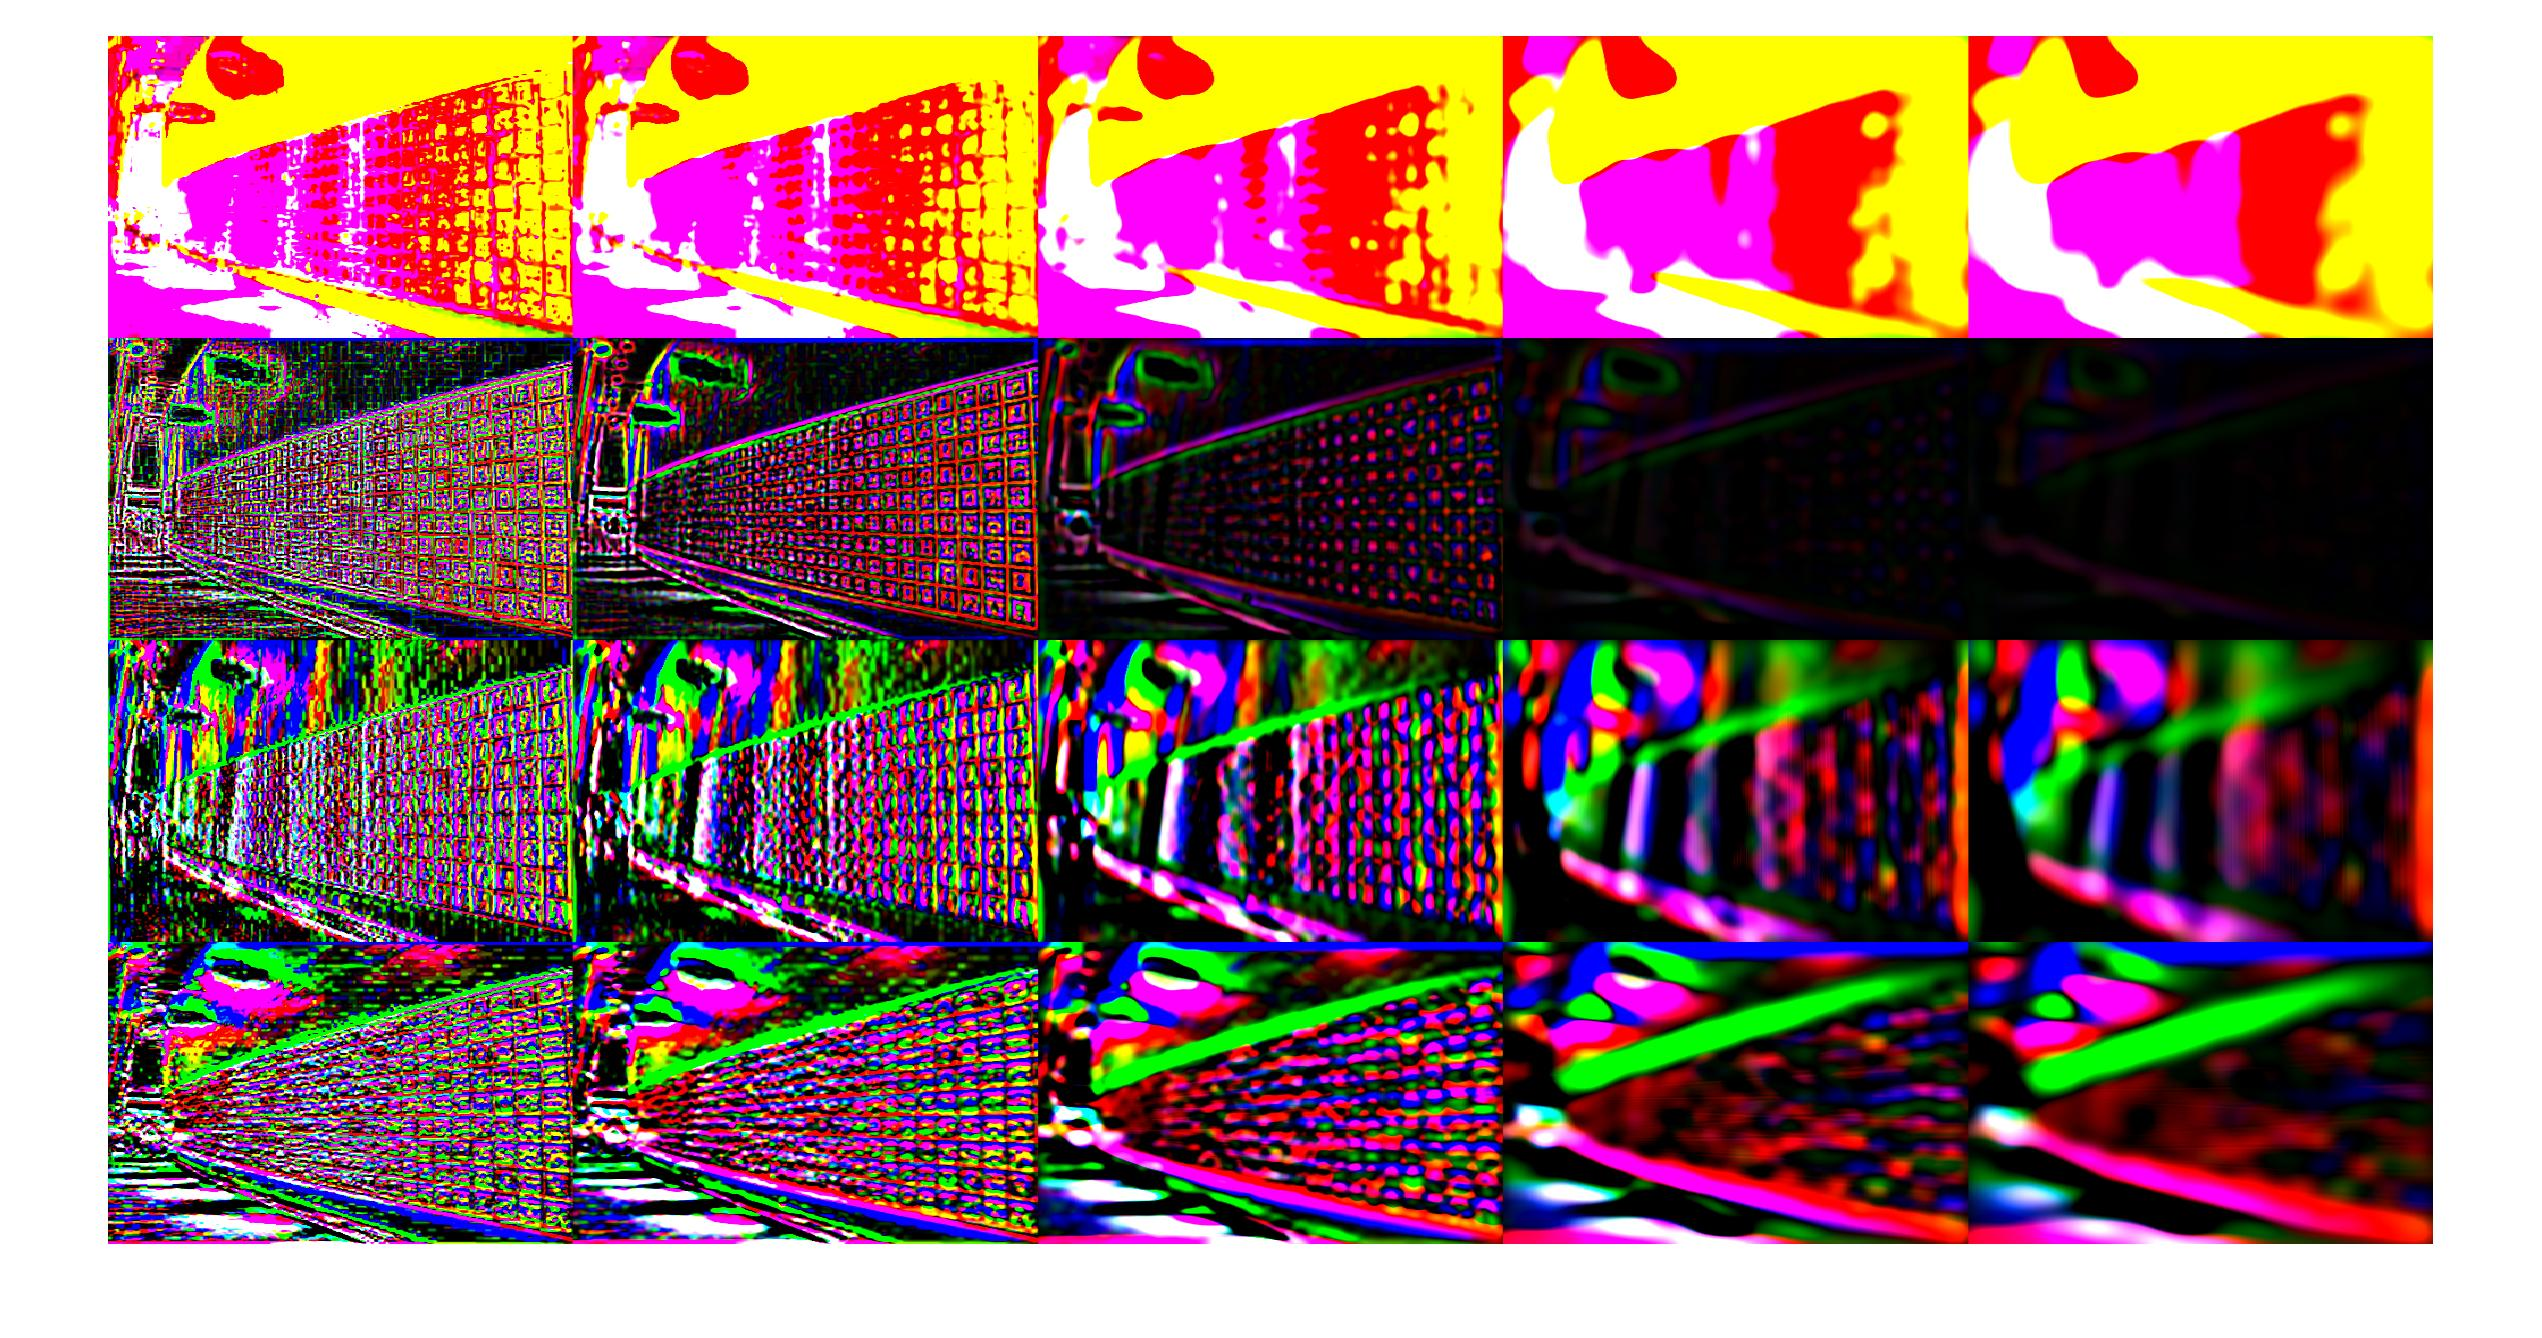
\includegraphics[width=\textwidth]{release/matlab/Montage4}
\begin{center}
	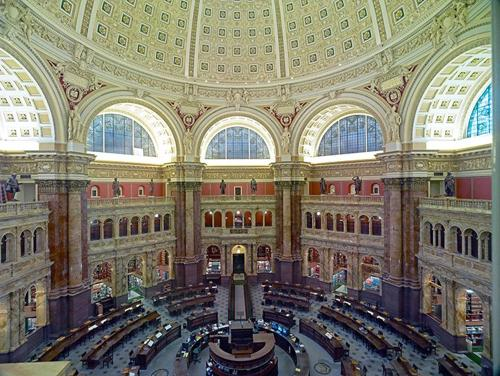
\includegraphics[width=11cm]{release/matlab/fig5}
\end{center}
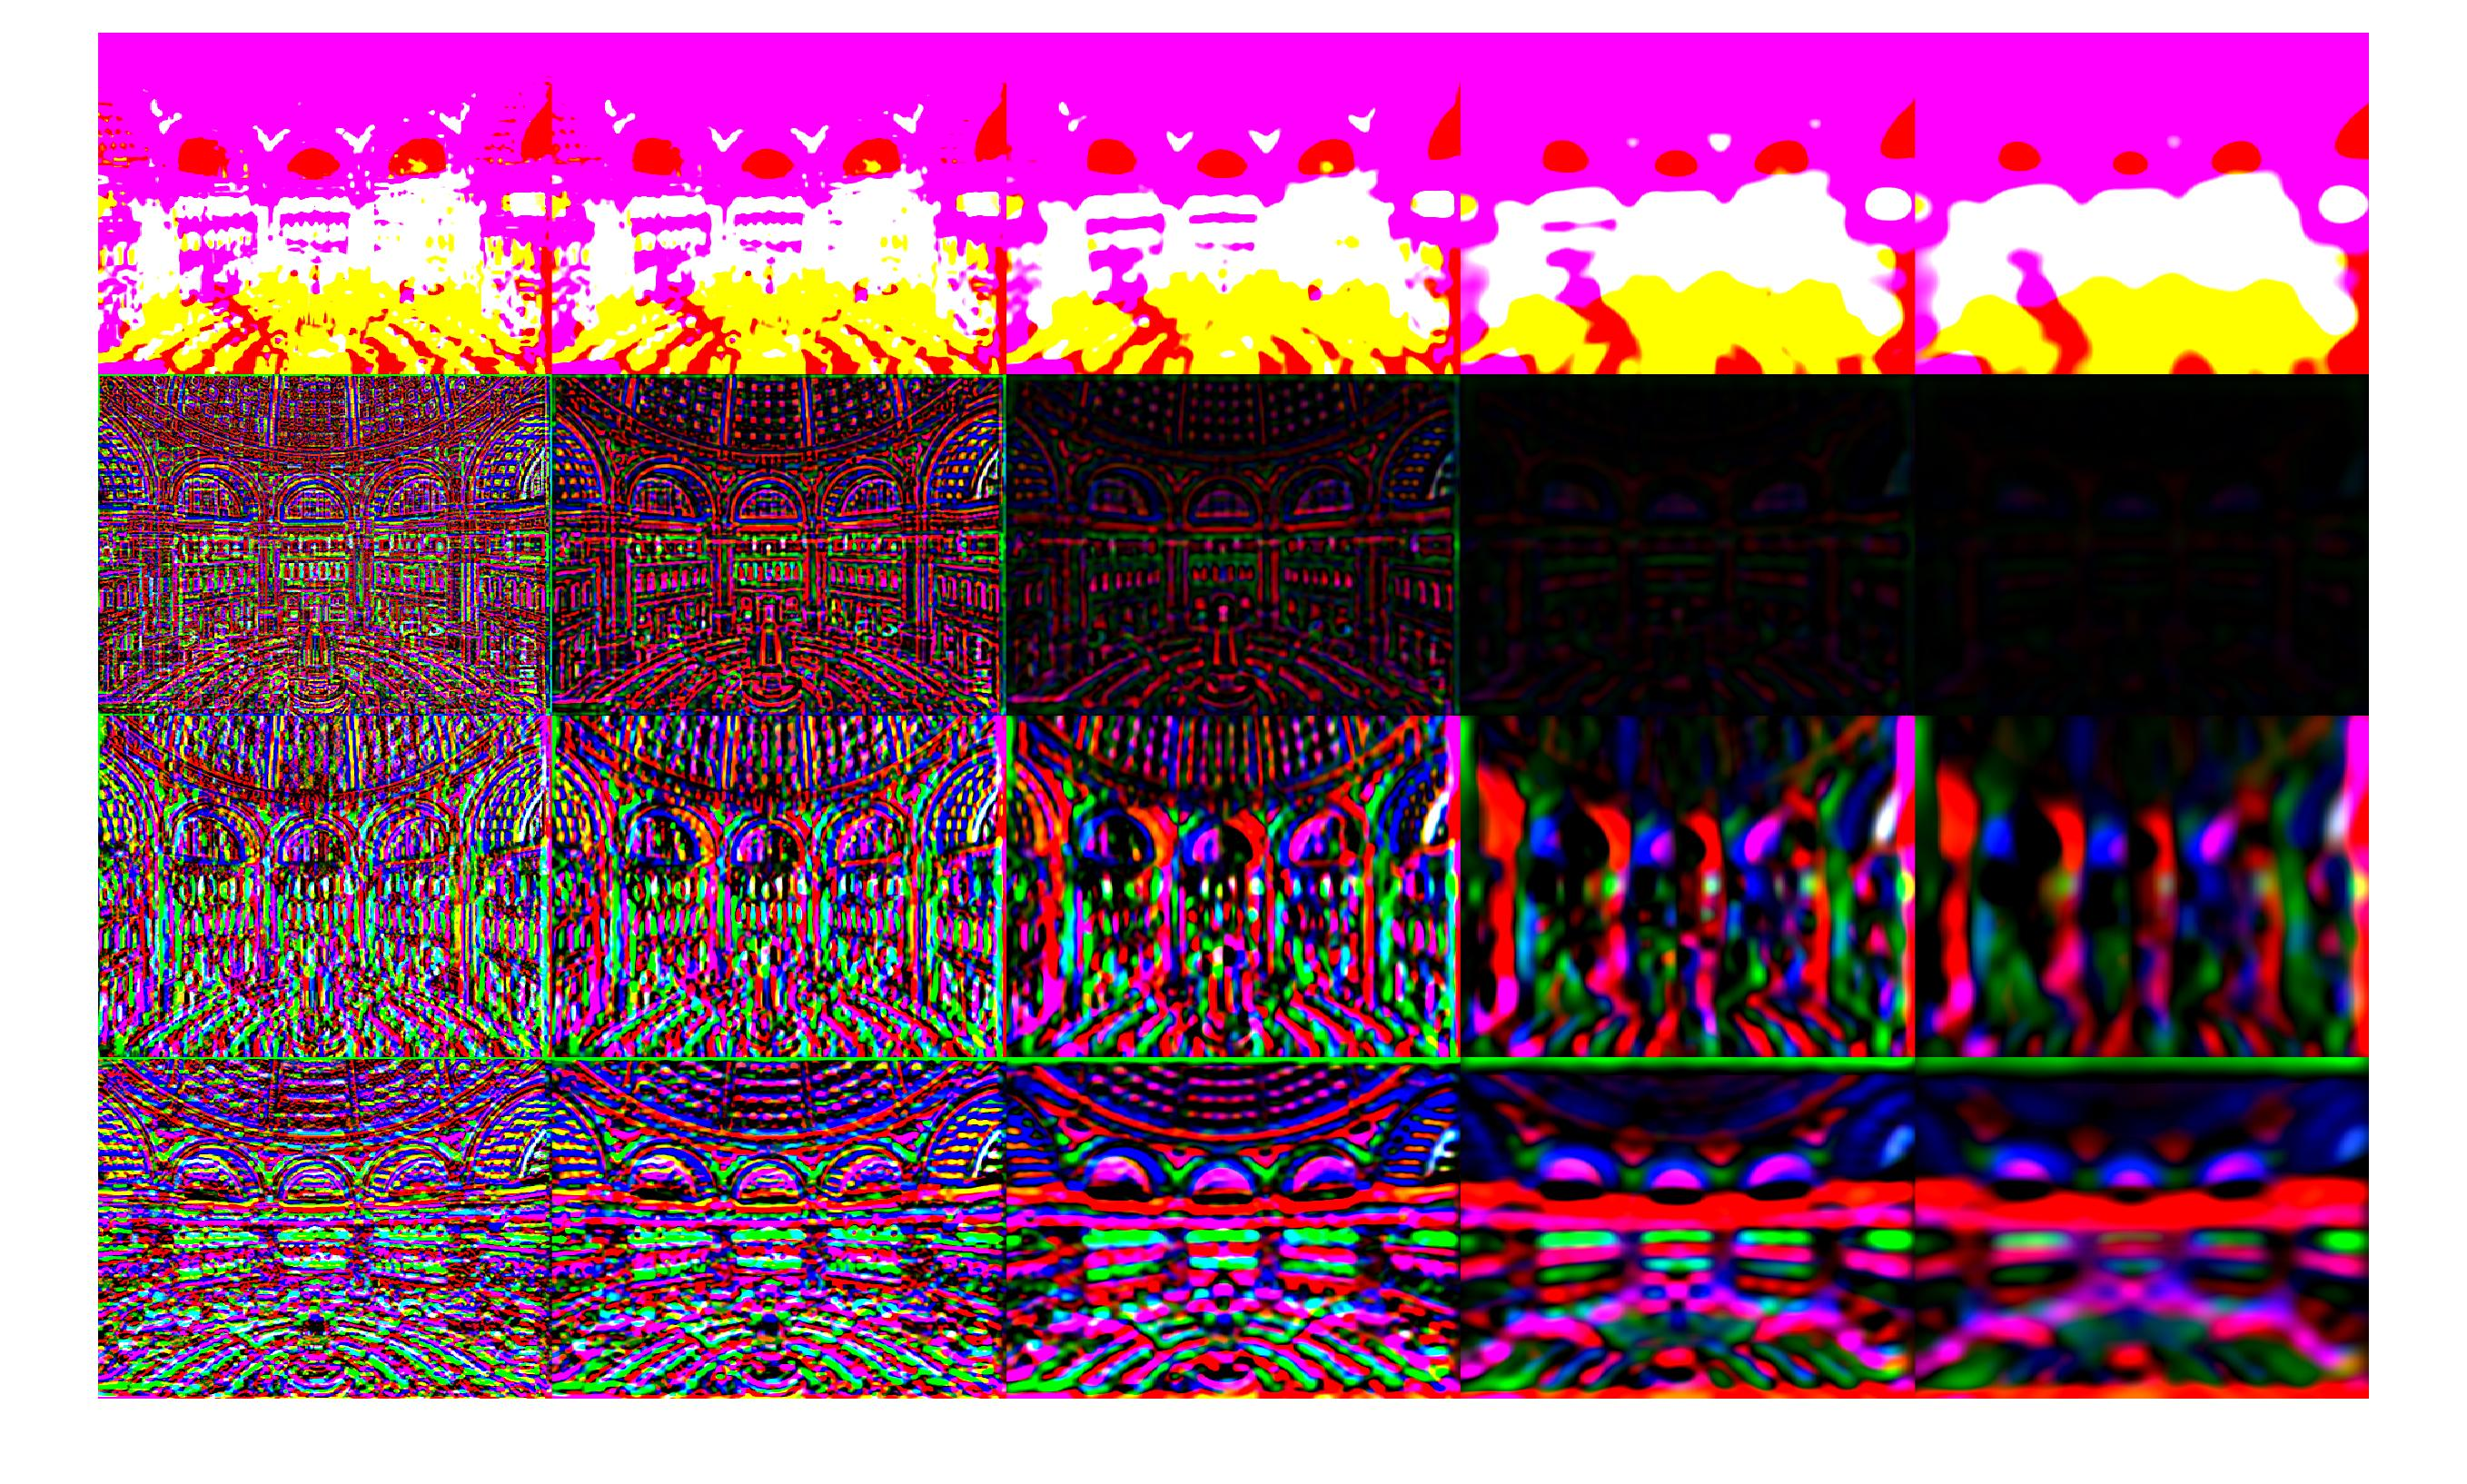
\includegraphics[width=\textwidth]{release/matlab/Montage5}
\begin{center}
	\includegraphics[width=11cm]{release/matlab/fig6}
\end{center}
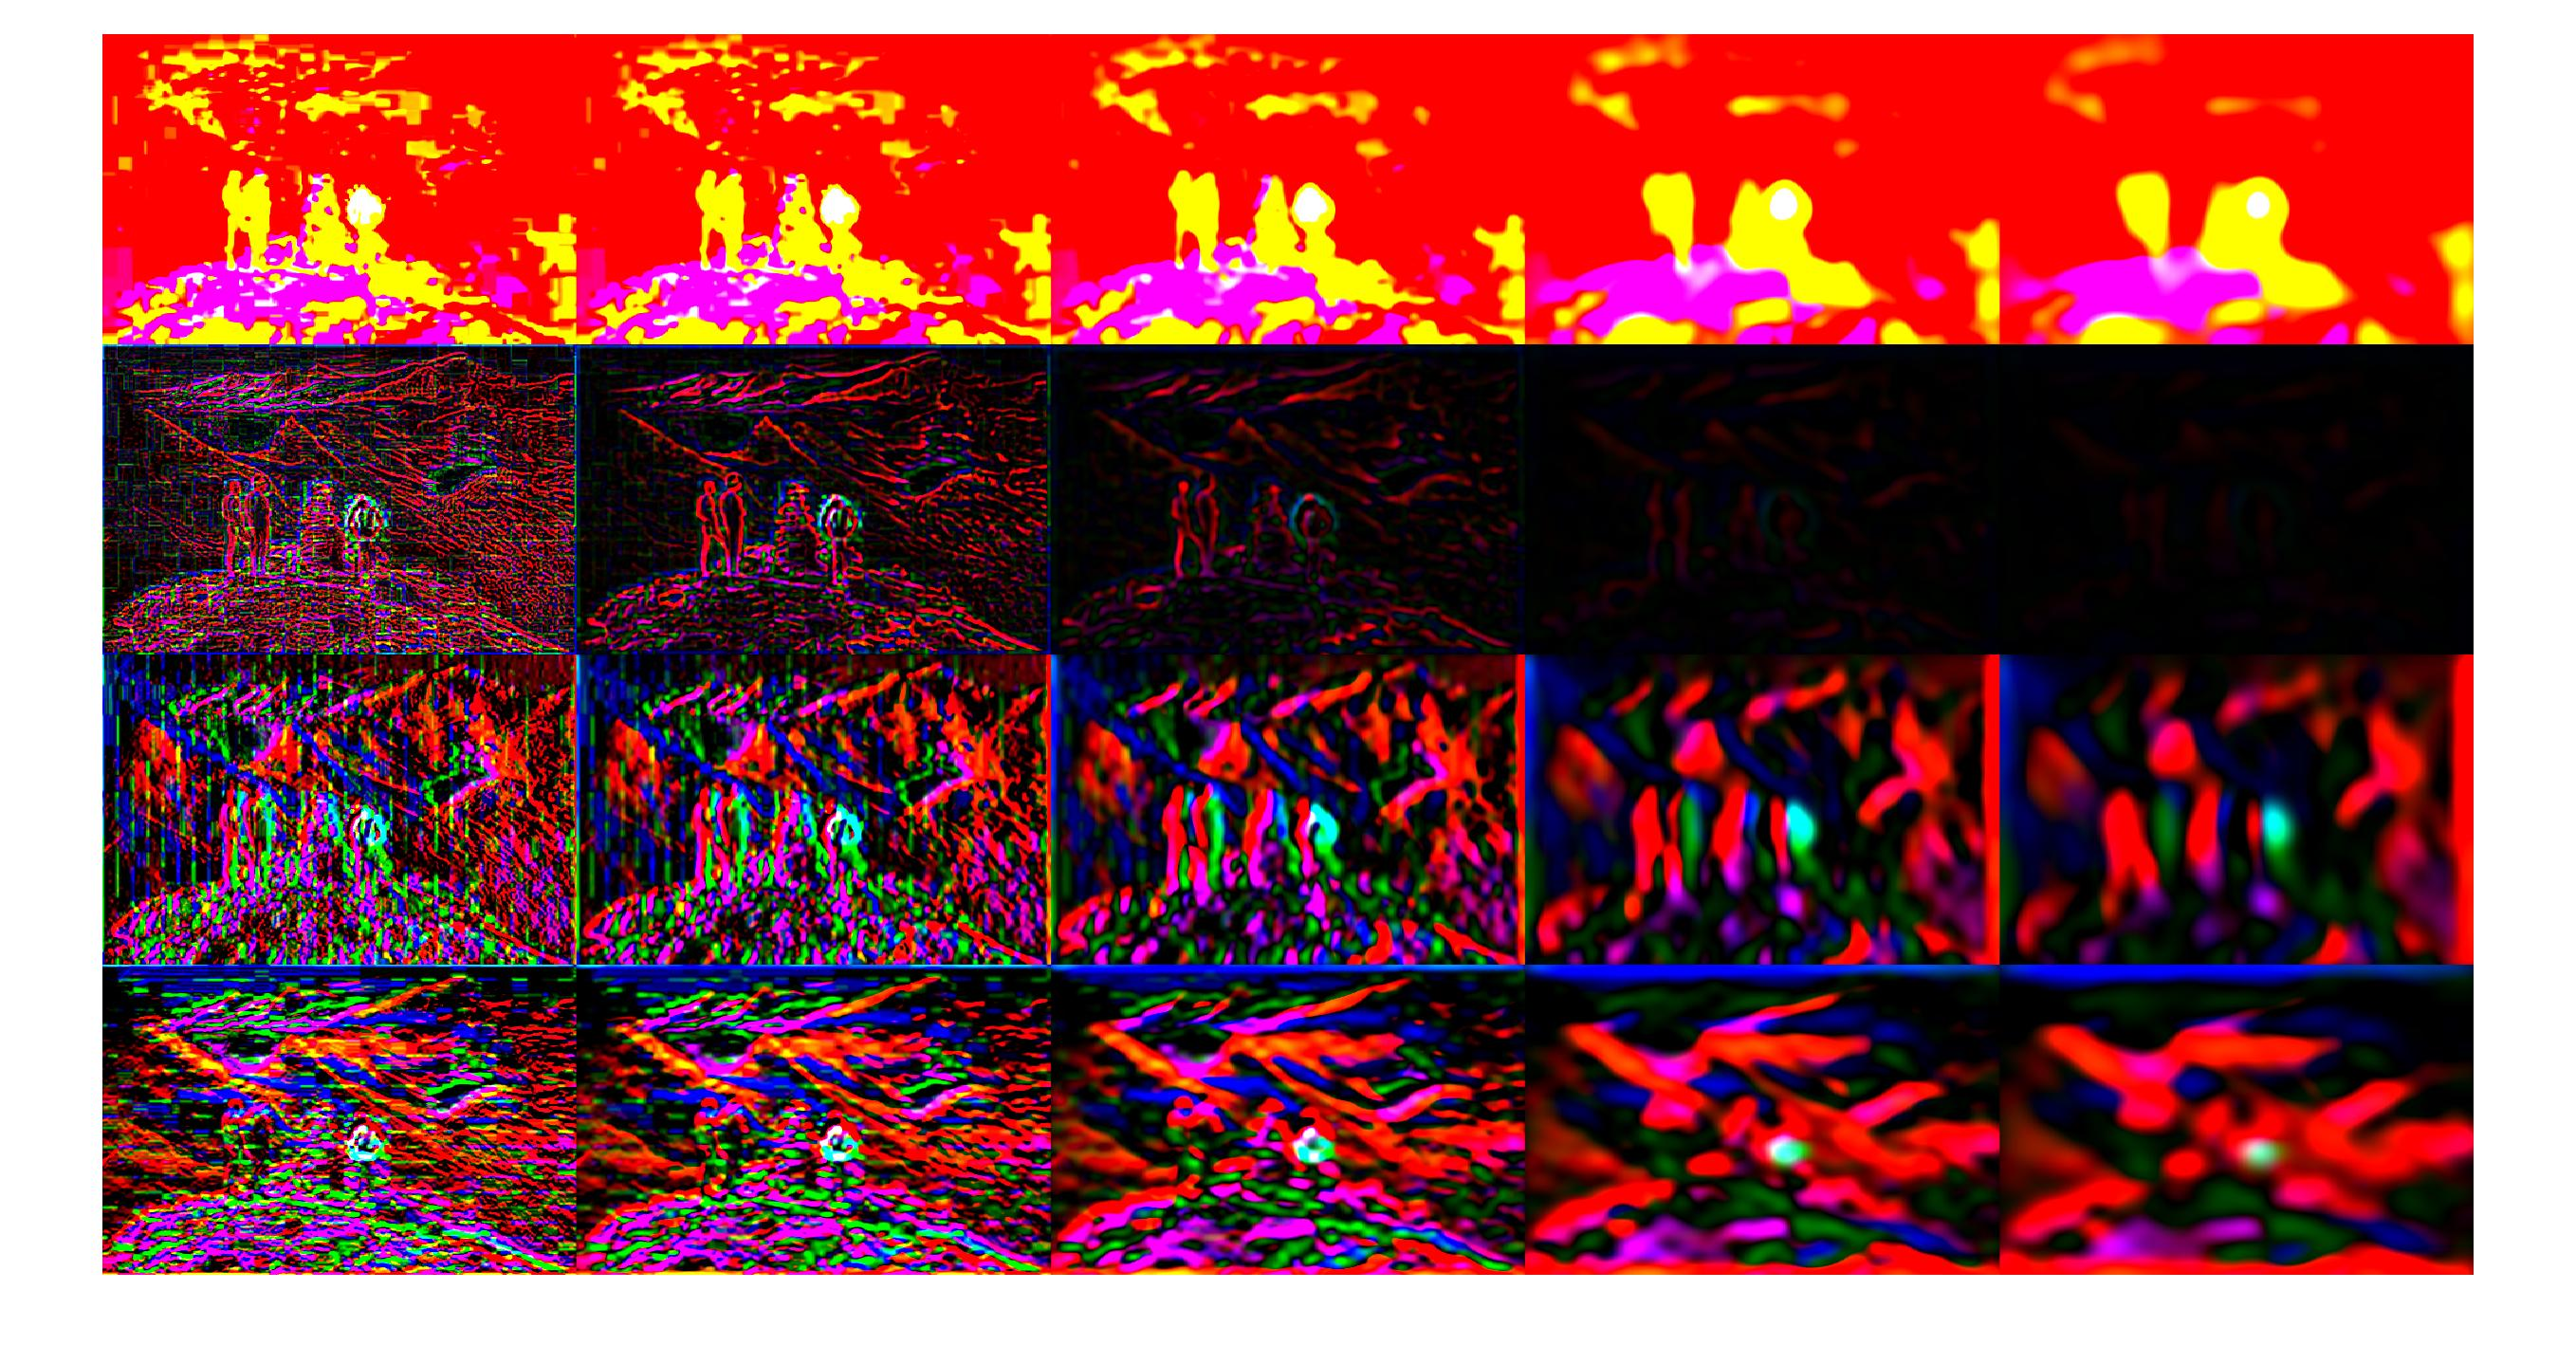
\includegraphics[width=\textwidth]{release/matlab/Montage6}

\section*{Problem 1.2}

An $\alpha$ value of 200 and \textit{K} of 256 are chosen.

\vfill
%\section*{Problem 1.3}
\begin{figure}
	\centering
	\begin{subfigure}{.5\textwidth}
		\centering
		\includegraphics[width=\textwidth]{release/matlab/fig4}
		\caption{Orginal Image}
		\label{fig:sub1}
	\end{subfigure}%
	\begin{subfigure}{.5\textwidth}
		\centering
		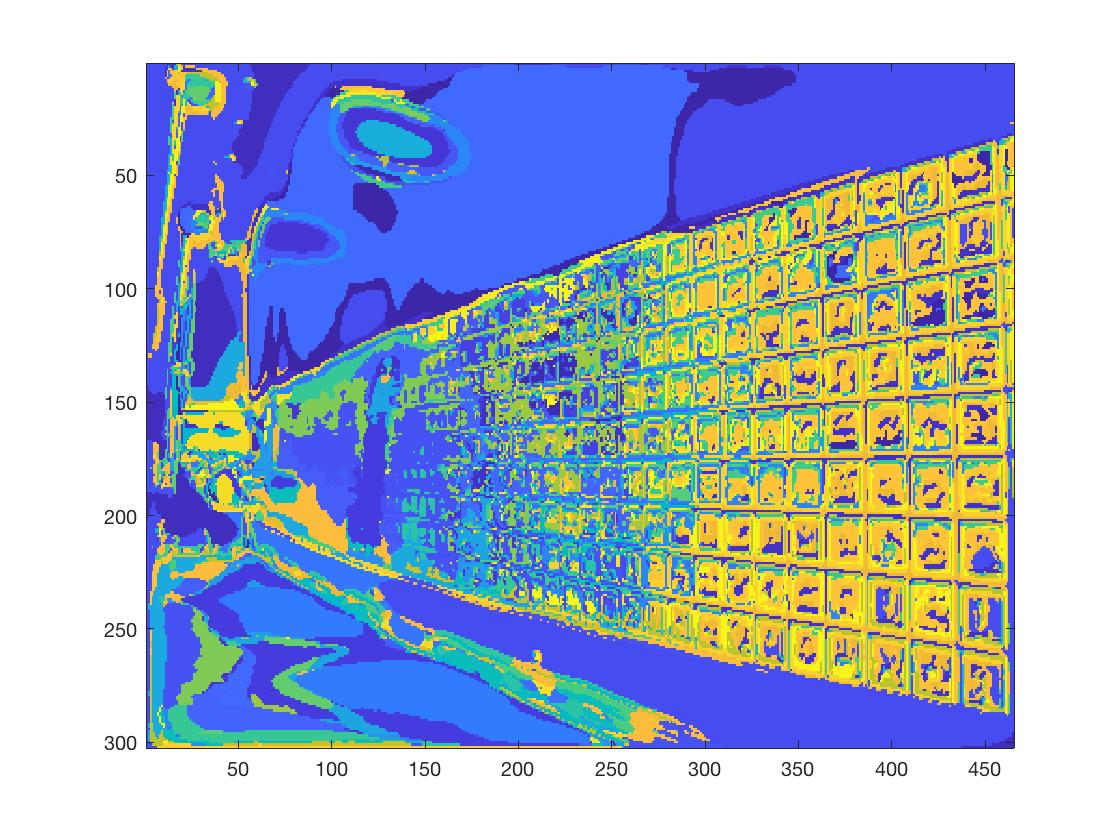
\includegraphics[width=\textwidth]{release/matlab/WordMap4}
		\caption{WordMap}
		\label{fig:sub2}
	\end{subfigure}
%	\caption{A figure with two subfigures}
%	\label{fig:test}
\end{figure}

\begin{figure}
	\centering
	\begin{subfigure}{.5\textwidth}
		\centering
		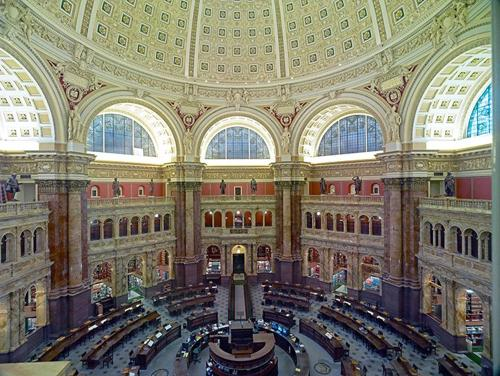
\includegraphics[width=\textwidth]{release/matlab/fig5}
		\caption{Orginal Image}
		\label{fig:sub1}
	\end{subfigure}%
	\begin{subfigure}{.5\textwidth}
		\centering
		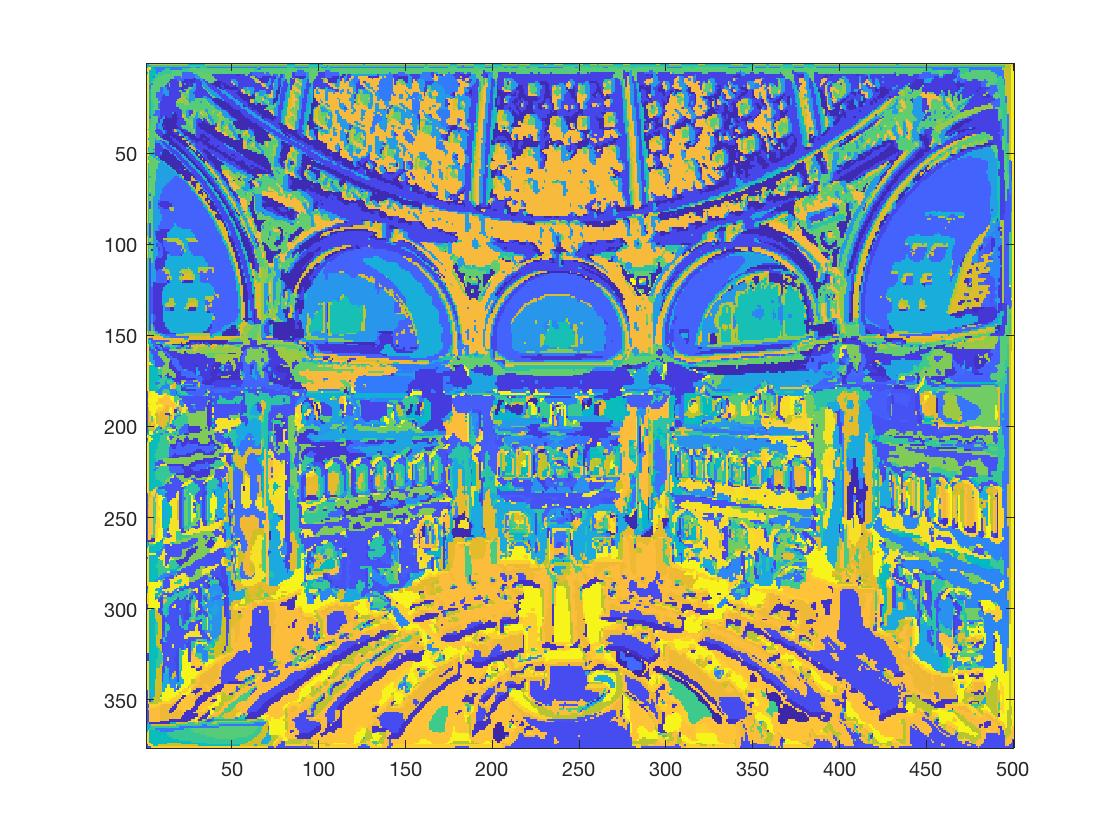
\includegraphics[width=\textwidth]{release/matlab/WordMap5}
		\caption{WordMap}
		\label{fig:sub2}
	\end{subfigure}
	%	\caption{A figure with two subfigures}
	%	\label{fig:test}
\end{figure}
\begin{figure}
	\centering
	\begin{subfigure}{.5\textwidth}
		\centering
		\includegraphics[width=\textwidth]{release/matlab/fig6}
		\caption{Orginal Image}
		\label{fig:sub1}
	\end{subfigure}%
	\begin{subfigure}{.5\textwidth}
		\centering
		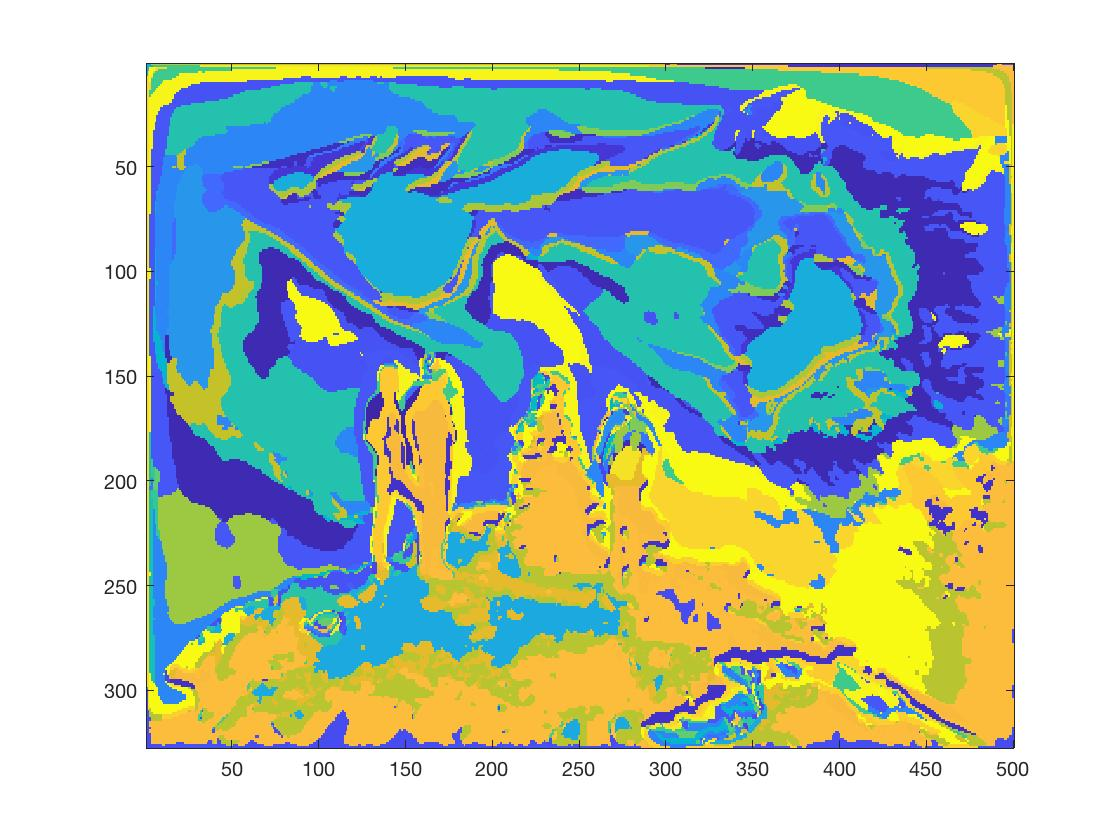
\includegraphics[width=\textwidth]{release/matlab/WordMap6}
		\caption{WordMap}
		\label{fig:sub2}
	\end{subfigure}
	%	\caption{A figure with two subfigures}
	%	\label{fig:test}
\end{figure}


\section*{Results}

\begingroup\makeatletter\def\@currenvir{verbatim}
\verbatim
Confusion Matrix":

8     1     1     5     5     0     0     0
0     3     2     3     9     0     1     2
0     0    17     0     2     1     0     0
2     1     0    13     3     0     0     1
2     1     4     1    12     0     0     0
0     1     2     0     3     6     8     0
1     0     0     0     0     3    16     0
1     2     6     4     1     3     0     3 

Accuracy: 0.487500
\end{verbatim}

%\verb|    
% 8     1     1     5     5     0     0     0
%0     3     2     3     9     0     1     2
%0     0    17     0     2     1     0     0
%2     1     0    13     3     0     0     1
%2     1     4     1    12     0     0     0
%0     1     2     0     3     6     8     0
%1     0     0     0     0     3    16     0
%1     2     6     4     1     3     0     3|



\end{document}
